\documentclass[tikz,border=10pt]{standalone}
\usepackage{tikz}
\usetikzlibrary{positioning,arrows.meta,shapes.geometric,calc,patterns,decorations.pathreplacing}

\begin{document}
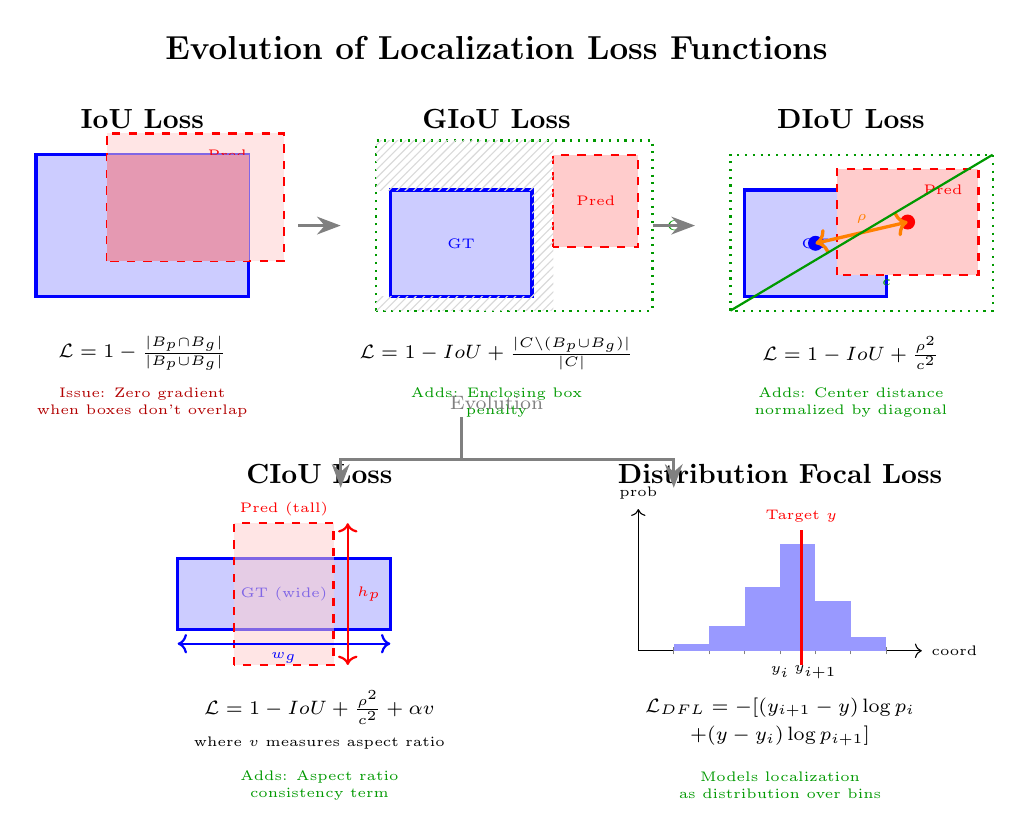
\begin{tikzpicture}[
    scale=0.9,
    every node/.style={font=\small}
]

% Title
\node[font=\bfseries\large] at (7,9) {Evolution of Localization Loss Functions};

% === IoU Loss (leftmost) ===
\begin{scope}[shift={(0,5)}]
\node[font=\bfseries] at (2,3) {IoU Loss};

% Ground truth box
\fill[blue!20] (0.5,0.5) rectangle (3.5,2.5);
\draw[blue, very thick] (0.5,0.5) rectangle (3.5,2.5);
\node[font=\tiny, blue] at (2,1.5) {GT};

% Predicted box (overlapping)
\fill[red!20, opacity=0.5] (1.5,1) rectangle (4,2.8);
\draw[red, thick, dashed] (1.5,1) rectangle (4,2.8);
\node[font=\tiny, red] at (3.2,2.5) {Pred};

% Intersection highlight
\fill[purple!40] (1.5,1) rectangle (3.5,2.5);

% Formula
\node[font=\scriptsize, align=center] at (2,-0.3) {$\mathcal{L} = 1 - \frac{|B_p \cap B_g|}{|B_p \cup B_g|}$};

% Issue annotation
\node[font=\tiny, red!70!black, align=center] at (2,-1) {Issue: Zero gradient\\when boxes don't overlap};
\end{scope}

% === GIoU Loss ===
\begin{scope}[shift={(5,5)}]
\node[font=\bfseries] at (2,3) {GIoU Loss};

% Ground truth box
\fill[blue!20] (0.5,0.5) rectangle (2.5,2);
\draw[blue, very thick] (0.5,0.5) rectangle (2.5,2);
\node[font=\tiny, blue] at (1.5,1.25) {GT};

% Predicted box (non-overlapping)
\fill[red!20] (2.8,1.2) rectangle (4,2.5);
\draw[red, thick, dashed] (2.8,1.2) rectangle (4,2.5);
\node[font=\tiny, red] at (3.4,1.85) {Pred};

% Enclosing box C
\draw[green!60!black, thick, dotted] (0.3,0.3) rectangle (4.2,2.7);
\node[font=\tiny, green!60!black] at (4.5,1.5) {C};

% Empty region annotation
\fill[pattern=north east lines, pattern color=gray!30] (2.5,0.3) rectangle (2.8,2.7);
\fill[pattern=north east lines, pattern color=gray!30] (0.3,2) rectangle (2.5,2.7);
\fill[pattern=north east lines, pattern color=gray!30] (0.3,0.3) rectangle (2.5,0.5);

% Formula
\node[font=\scriptsize, align=center] at (2,-0.3) {$\mathcal{L} = 1 - IoU + \frac{|C \setminus (B_p \cup B_g)|}{|C|}$};

% Improvement
\node[font=\tiny, green!60!black, align=center] at (2,-1) {Adds: Enclosing box\\penalty};
\end{scope}

% === DIoU Loss ===
\begin{scope}[shift={(10,5)}]
\node[font=\bfseries] at (2,3) {DIoU Loss};

% Ground truth box
\fill[blue!20] (0.5,0.5) rectangle (2.5,2);
\draw[blue, very thick] (0.5,0.5) rectangle (2.5,2);
\node[font=\tiny, blue] at (1.5,1.25) {GT};

% Predicted box
\fill[red!20] (1.8,0.8) rectangle (3.8,2.3);
\draw[red, thick, dashed] (1.8,0.8) rectangle (3.8,2.3);
\node[font=\tiny, red] at (3.3,2) {Pred};

% Center points
\fill[blue] (1.5,1.25) circle (3pt);
\fill[red] (2.8,1.55) circle (3pt);

% Distance line
\draw[orange, very thick, <->] (1.5,1.25) -- (2.8,1.55);
\node[font=\tiny, orange] at (2.15,1.6) {$\rho$};

% Enclosing box diagonal
\draw[green!60!black, thick, dotted] (0.3,0.3) rectangle (4,2.5);
\draw[green!60!black, thick] (0.3,0.3) -- (4,2.5);
\node[font=\tiny, green!60!black] at (2.5,0.7) {$c$};

% Formula
\node[font=\scriptsize, align=center] at (2,-0.3) {$\mathcal{L} = 1 - IoU + \frac{\rho^2}{c^2}$};

% Improvement
\node[font=\tiny, green!60!black, align=center] at (2,-1) {Adds: Center distance\\normalized by diagonal};
\end{scope}

% === CIoU Loss (bottom left) ===
\begin{scope}[shift={(2.5,0)}]
\node[font=\bfseries] at (2,3) {CIoU Loss};

% Ground truth box (wide)
\fill[blue!20] (0,0.8) rectangle (3,1.8);
\draw[blue, very thick] (0,0.8) rectangle (3,1.8);
\node[font=\tiny, blue] at (1.5,1.3) {GT (wide)};

% Predicted box (different aspect ratio)
\fill[red!20, opacity=0.5] (0.8,0.3) rectangle (2.2,2.3);
\draw[red, thick, dashed] (0.8,0.3) rectangle (2.2,2.3);
\node[font=\tiny, red] at (1.5,2.5) {Pred (tall)};

% Aspect ratio indicators
\draw[blue, thick, <->] (0,0.6) -- (3,0.6);
\node[font=\tiny, blue] at (1.5,0.4) {$w_g$};

\draw[red, thick, <->] (2.4,0.3) -- (2.4,2.3);
\node[font=\tiny, red] at (2.7,1.3) {$h_p$};

% Formula
\node[font=\scriptsize, align=center] at (2,-0.3) {$\mathcal{L} = 1 - IoU + \frac{\rho^2}{c^2} + \alpha v$};
\node[font=\tiny, align=center] at (2,-0.8) {where $v$ measures aspect ratio};

% Improvement
\node[font=\tiny, green!60!black, align=center] at (2,-1.4) {Adds: Aspect ratio\\consistency term};
\end{scope}

% === DFL (bottom right) ===
\begin{scope}[shift={(9,0)}]
\node[font=\bfseries] at (2,3) {Distribution Focal Loss};

% Distribution visualization
\draw[->] (0,0.5) -- (4,0.5) node[right, font=\tiny] {coord};
\draw[->] (0,0.5) -- (0,2.5) node[above, font=\tiny] {prob};

% Discrete bins
\foreach \x in {0.5,1,1.5,2,2.5,3,3.5} {
    \draw[gray] (\x,0.45) -- (\x,0.55);
}

% Distribution bars (Gaussian-like centered around 2)
\fill[blue!40] (0.5,0.5) rectangle (1,0.6);
\fill[blue!40] (1,0.5) rectangle (1.5,0.85);
\fill[blue!40] (1.5,0.5) rectangle (2,1.4);
\fill[blue!40] (2,0.5) rectangle (2.5,2.0);
\fill[blue!40] (2.5,0.5) rectangle (3,1.2);
\fill[blue!40] (3,0.5) rectangle (3.5,0.7);

% True coordinate marker
\draw[red, very thick] (2.3,0.3) -- (2.3,2.2);
\node[font=\tiny, red] at (2.3,2.4) {Target $y$};

% Key bins
\node[font=\tiny] at (2,0.2) {$y_i$};
\node[font=\tiny] at (2.5,0.2) {$y_{i+1}$};

% Formula
\node[font=\scriptsize, align=center] at (2,-0.3) {$\mathcal{L}_{DFL} = -[(y_{i+1}-y)\log p_i$};
\node[font=\scriptsize, align=center] at (2,-0.7) {$+ (y-y_i)\log p_{i+1}]$};

% Description
\node[font=\tiny, green!60!black, align=center] at (2,-1.4) {Models localization\\as distribution over bins};
\end{scope}

% === Evolution arrows ===
\draw[-{Stealth[length=3mm]}, very thick, gray] (4.2,6.5) -- (4.8,6.5);
\draw[-{Stealth[length=3mm]}, very thick, gray] (9.2,6.5) -- (9.8,6.5);
\draw[-{Stealth[length=3mm]}, very thick, gray] (6.5,3.8) -- (6.5,3.2) -- (4.8,3.2) -- (4.8,2.8);
\draw[-{Stealth[length=3mm]}, very thick, gray] (6.5,3.2) -- (9.5,3.2) -- (9.5,2.8);

% Timeline label
\node[font=\scriptsize, gray] at (7,4) {Evolution};

\end{tikzpicture}
\end{document}
